\documentclass{beamer}
\usepackage{beamerthemesplit} 
\usetheme{Warsaw}
\usepackage[spanish]{babel} 
\usepackage{ucs}
\usepackage[utf8]{inputenc}

\usepackage{amsthm}
\usepackage{amsmath}
\usepackage{amssymb}
\usepackage{esint}

\usepackage{siunitx}
\usepackage{physics}
\usepackage{graphicx}
\usepackage{xcolor}
\setbeamertemplate{navigation symbols}{}

\begin{document}
\title{La entropía de los agujeros negros y el problema de Hagedorn}  
\author{John Liu Anta\\
        Tutor: Miguel Ángel Ramos Osorio}
\date{\today} 
\frame{\titlepage} 

\begin{frame}
  \frametitle{Objetivo}
  \begin{itemize}
    \item Temperatura Hagedorn: temperatura a partir de la cual la descripción termodinámica de cuerdas parece
      perder sentido
    \item  Muy estudiada en espacios planos
    \item  ¿Qué pasa si hay curvatura debido a la gravedad?
    \item Para agujeros negros, encontramos que la temperatura de Hagedorn coincide con la 
      temperatura de Hawking
  \end{itemize}
\end{frame}


\begin{frame}
  \frametitle{Motivación}
  \begin{itemize}
    \item     Teoría de cuerdas: Consideramos una teoría cuántica relativista en la cual las entidades fundamentales
      son cuerdas, no partículas
    \item Cuerdas bosónicas y cuerdas supersimétricas (incluyen fermiones)
    \item  La cuerdas se pueden excitar. Cada excitación de la cuerda corresponde a un estado
  \end{itemize}

\end{frame}

\begin{frame}
  \frametitle{Temperatura de Hagedorn}
\begin{itemize}
  \item Hay distintos estados de vibración con la misma energía
  \item Densidad de estados $\omega(E)$: $\omega(E)\delta E$ número de estados en el intervalo $(E,E+\delta E)$
  \item Para cuerdas
    \begin{equation*}
      \omega(E) \approx \frac{e^{\beta_H E}}{E^{D/2+1}}
    \end{equation}
  \item Temperatura de Hagedorn para cuerdas bosónicas cerradas
    \begin{equation*}
      \beta_H = \frac{1}{k_B T_H} =  4\pi\sqrt{\alpha'}, \qquad
      \alpha'=\frac{1}{2\pi \cdot \text{tensión}}
    \end{equation}

    \begin{equation*}
      T_H \approx \SI{e30}{K} \quad !
    \end{equation}
\end{itemize}
\end{frame}

\begin{frame}
  \frametitle{Temperatura de Hagedorn}
\begin{itemize}
  \item Cuerda en contacto con una fuente de calor a temperatura $\beta$
  \item Probabilidad de que un estado con energía $E$ esté ocupado es
    \begin{equation*}
      p(E)=\frac{e^{-\beta E}}{Z},  \quad \text{Z: función de partición (normalización)}
    \end{equation}
\end{itemize}
\end{frame}

\begin{frame}
  \frametitle{Temperatura de Hagedorn}
\begin{itemize}
  \item Cuerda en contacto con una fuente de calor a temperatura $\beta$
  \item Probabilidad de que un estado con energía $E$ esté ocupado es
    \begin{equation*}
      p(E)=\frac{e^{-\beta E}}{Z},  \quad \text{Z: función de partición (normalización)}
    \end{equation}
  \item ¡PROBLEMA! Si $T>T_H$, la probabilidad de que la cuerda tenga energía $E$ crece con $E$
    \begin{equation*}
      p(E)\omega(E) \approx e^{(\beta_H-\beta) E}
    \end{equation}
    y $Z$ diverge
  \item Divergencia debida a los estados muy masivos
\end{itemize}
\end{frame}

\begin{frame}
  \frametitle{¿Qué ocurre cerca de la temperatura de Hagedorn?}
  \begin{itemize}
    \item ¿Temperatura límite?
    \item Las cuerdas tiende a unirse en una sola cuerda muy larga
      \begin{center}
      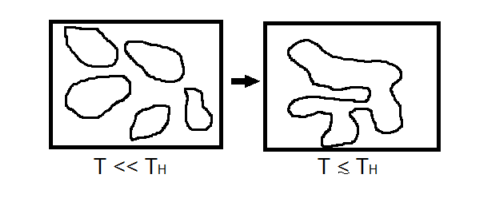
\includegraphics[width=0.5\textwidth]{long.png}
      \end{center}
    \item La energía libre también diverge
      \begin{equation*}
        F(\beta) = E - TS 
      \end{equation}
  \end{itemize}
\end{frame}

\begin{frame}
  \frametitle{Enfoque alternativo}
  \begin{itemize}
    \item Suponemos un tiempo imaginario con periodo $\beta$
    \item Calculamos la energía libre mediante la integral de camino:
      hacemos una "suma" sobre todas las posibles configuraciones de la cuerda
    \item Estado que se enrolla en el tiempo causa la divergencia de Hagedorn
      \begin{center}
      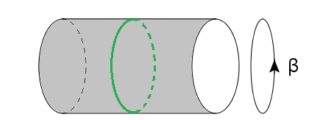
\includegraphics[width=0.5\textwidth]{string.png}
      \end{center}
      \begin{equation*}
        m^2 = \frac{\beta^2-\beta_H^2}{4\pi^2\alpha'^2}
      \end{equation}
    \item Pasa a tener masa imaginaria si $T>T_H$ (estado taquiónico)
  \end{itemize}
\end{frame}
\begin{frame}
  \frametitle{Radiación de Hawking}
  \begin{itemize}
    \item Horizonte de sucesos: superficie de la cual nada puede escapar
    \item Un agujero negro debería emitir radiación de cuerpo negro a la temperatura de Hawking
      \begin{equation*}
  T_{haw}=\frac{\hbar c^3}{8\pi k_B GM}
      \end{equation}
    \item Temperatura muy pequeña, para un agujero negro con la masa del Sol, \SI{60}{nK}.
  \end{itemize}
\end{frame}


\begin{frame}
  \frametitle{Cuerdas cerca de agujeros negros}
  \begin{itemize}
    \item Asumimos que la divergencia de Hagedorn se sigue debiendo al estado taquiónico
    \item Calculamos la integral de camino asociada a un campo taquiónico $T$
    \item Partimos de la acción
\begin{equation*}
  S=\frac{1}{2}\int d^d x\sqrt G e^{-2\Phi}  \qty(G^{\mu\nu}\partial_\mu T\partial_\nu T+m^2T^2),
\end{equation}
    \item Haciendo un desarrollo de Fourier e integrando por partes
\begin{equation*}
  S \approx \int d^{d-1} x \sqrt G e^{-2\Phi} T^* \widehat O T
\end{equation}
donde       
\begin{equation*}
\widehat O  = - G^{ij}\nabla_i \partial_j-G^{ij}\frac{\partial_j \sqrt{G_{00}}}{\sqrt G_{00}}\partial_i + m^2_{efectiva}(x)
\end{equation}
  \end{itemize}
\end{frame}

\begin{frame}
  \frametitle{Cuerdas cerca de agujeros negros}
  \begin{itemize}
      
    \item La integral de camino de la acción obtenida es
      \begin{equation*}
        Z = \int \mathcal D T e^{-S/\hbar} = \det \widehat O ^{-1}
      \end{equation}
    \item La energía libre es
      \begin{gather*}
        F = -\frac{1}{\beta}\ln Z = \frac{1}{\beta}\Tr \ln \widehat O \\
        F=-\frac{1}{\beta}\int_0^\infty \frac{dT}{T} \Tr e^{-T\widehat O}
      \end{gather}
    \item  Sustituimos $\widehat O$ para las proximidades de un agujero negro (de Schwarzschild) y
      buscamos sus valores propios
      \begin{equation*}
        ds^2 = \frac{\rho^2}{(4GM)^2} d\tau^2 +d\rho^2 +d\mathbf x_\perp ^2
      \end{equation}
      \begin{equation*}
        \widehat O = -\partial_\rho^2-\frac{1}{\rho}\partial_\rho-\frac{2}{\alpha'}+\frac{\beta^2}{4\pi^2 \alpha'^2}\frac{\rho^2}{(4GM)^2}
      \end{equation}

  \end{itemize}
\end{frame}

\begin{frame}
  \frametitle{Cuerdas cerca de agujeros negros}
  \begin{itemize}
    \item  Los valores propios son 
      \begin{equation*}
        \lambda_n=\frac{\beta(1+2n)}{(4GM)^2} - 2\pi
      \end{equation} 
      
      \begin{gather*}
        F \sim -\frac{1}{\beta}\int_0^\infty \frac{dT}{T}  \qty(\frac{1}{T^4}) e^{T\frac{c^3}{4GM}\qty(\beta_{haw}-\beta)}
      \end{gather}
      
    \item La divergencia de la energía libre se produce a la temperatura de Hawking
      \begin{equation*}
        T_{H} =  T_{haw}
      \end{equation}

  \end{itemize}
\end{frame}

\begin{frame}
  \frametitle{Entropía de agujeros negros}
  \begin{itemize}
    \item Un observador externo percibiría que la materia que ha atravesado el horizonte
      se acerca eternamente al horizonte sin cruzarlo. Nunca se alcanza el equilibrio
    \item Se podría acumular una cantidad infinita de materia (información) en el horizonte
    \item No sucede lo mismo con cuerdas. La función de onda es
      \begin{equation*}
        \psi(\rho) \sim e^{-\frac{\rho^2}{2L^2}}
      \end{equation}
    \item  Las cuerdas alcanzan el equilibrio en el entorno del agujero negro
      \begin{center}
      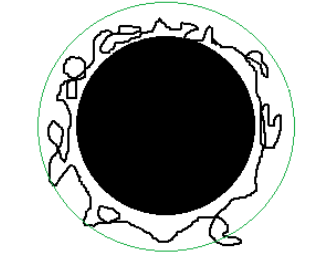
\includegraphics[width=0.3\textwidth]{bh.png}
      \end{center}
  \end{itemize}
\end{frame}

\begin{frame}
  \frametitle{Entropía de agujeros negros}
  \begin{itemize}
    \item Supongamos que cae una cuerda con energía $\delta E$ al agujero negro
      \begin{gather*}
        \delta S =\delta (k_B \ln \omega) =  \frac{\delta E}{T_H}\\
        \delta S =  c^2\frac{\delta M}{T_{haw}}  = \frac{8\pi k_B GM}{\hbar c}\delta M
      \end{gather}
    \item Integrando, recuperamos la  entropía de Bekenstein-Hawking
      \begin{equation*}
        S=k_B\frac{c^3 A}{4\hbar G},
      \end{equation}
    proporcional al área del agujero negro $A=4\pi \qty(\frac{2GM}{c^2})^2$
  \end{itemize}
\end{frame}


\begin{frame}
  \frametitle{Conclusión}
  \begin{itemize}
    \item Cálculos con mayor rigor
      \begin{itemize}
        \item Correcciones a orden superior
        \item Geometrías más generales
      \end{itemize}
    \item Cálculo de la entropía con branas (Strominger y Vafa)
    \item Problema de la información, fuzzballs, firewalls\dots
  \end{itemize}
\end{frame}

\end{frame}
\begin{frame}
  \begin{center}
  \Large{GRACIAS POR VUESTRA ATENCIÓN}
  \end{center}
\end{frame}

\end{frame}
\end{document}

